\begin{figure}[H]
\centering
\includegraphics[page=6,width=0.33\textwidth]{\FCNCFigures/xTFW/showFake/NOMINAL/reg2mtau1b2jos_vetobtagwp70_highmet/tautaumass.pdf}
\put(-30, 80){\textbf{(a1)}}
\includegraphics[page=6,width=0.33\textwidth]{\FCNCFigures/xTFW/showFake/NOMINAL/reg2mtau1b2jos_vetobtagwp70_highmet/ttvismass.pdf}
\put(-30, 80){\textbf{(a2)}}
\includegraphics[page=6,width=0.33\textwidth]{\FCNCFigures/xTFW/showFake/NOMINAL/reg2mtau1b2jos_vetobtagwp70_highmet/t1mass.pdf}
\put(-70, 70){\textbf{(a3)}}
\\
\includegraphics[page=6,width=0.33\textwidth]{\FCNCFigures/xTFW/showFake/NOMINAL/reg2mtau1b3jos_vetobtagwp70_highmet/tautaumass.pdf}
\put(-30, 80){\textbf{(b1)}}
\includegraphics[page=6,width=0.33\textwidth]{\FCNCFigures/xTFW/showFake/NOMINAL/reg2mtau1b3jos_vetobtagwp70_highmet/ttvismass.pdf}
\put(-30, 80){\textbf{(b2)}}
\includegraphics[page=6,width=0.33\textwidth]{\FCNCFigures/xTFW/showFake/NOMINAL/reg2mtau1b3jos_vetobtagwp70_highmet/drtautau.pdf}
\put(-70, 70){\textbf{(b3)}}
\\
\caption{ The BDT input distributions for the background and merged signal in the $t_h\thadhad$-2j (a1-3), $t_h\thadhad$-3j (b1-3)}% The Kolmogorov Test values for the training and testing BDT distributions are also indicated.
\label{fig:mva_input_hadhad}
\end{figure}

\begin{figure}[H]
\centering
\includegraphics[page=6,width=0.33\textwidth]{\FCNCFigures/tthML/showFake/faketau/postfit/NOMINAL/reg1l1tau1b2j_os_vetobtagwp70_highmet/x1fit.pdf}
\put(-30, 80){\textbf{(a1)}}
\includegraphics[page=6,width=0.33\textwidth]{\FCNCFigures/tthML/showFake/faketau/postfit/NOMINAL/reg1l1tau1b2j_os_vetobtagwp70_highmet/x2fit.pdf}
\put(-30, 80){\textbf{(a2)}}
\includegraphics[page=6,width=0.33\textwidth]{\FCNCFigures/tthML/showFake/faketau/postfit/NOMINAL/reg1l1tau1b2j_os_vetobtagwp70_highmet/ttvismass.pdf}
\put(-70, 70){\textbf{(a3)}}
\\
\includegraphics[page=6,width=0.33\textwidth]{\FCNCFigures/tthML/showFake/faketau/postfit/NOMINAL/reg1l1tau1b3j_os_vetobtagwp70_highmet/x1fit.pdf}
\put(-30, 80){\textbf{(b1)}}
\includegraphics[page=6,width=0.33\textwidth]{\FCNCFigures/tthML/showFake/faketau/postfit/NOMINAL/reg1l1tau1b3j_os_vetobtagwp70_highmet/x2fit.pdf}
\put(-30, 80){\textbf{(b2)}}
\includegraphics[page=6,width=0.33\textwidth]{\FCNCFigures/tthML/showFake/faketau/postfit/NOMINAL/reg1l1tau1b3j_os_vetobtagwp70_highmet/ttvismass.pdf}
\put(-70, 70){\textbf{(b3)}}
\\
\caption{ The BDT input distributions for the background and merged signal in the $t_h\tlhad$-2j (a1-3), $t_h\tlhad$-3j (b1-3). }% The Kolmogorov Test values for the training and testing BDT distributions are also indicated.
\label{fig:mva_input_lephad}
\end{figure}

\begin{figure}[H]
\centering
\includegraphics[page=6,width=0.33\textwidth]{\FCNCFigures/tthML/showFake/faketau/postfit/NOMINAL/reg1l2tau1bnj_os/ttvismass.pdf}
\put(-30, 80){\textbf{(a1)}}
\includegraphics[page=6,width=0.33\textwidth]{\FCNCFigures/tthML/showFake/faketau/postfit/NOMINAL/reg1l2tau1bnj_os/drtautau.pdf}
\put(-30, 80){\textbf{(a2)}}
\includegraphics[page=6,width=0.33\textwidth]{\FCNCFigures/tthML/showFake/faketau/postfit/NOMINAL/reg1l2tau1bnj_os/t2vismass.pdf}
\put(-70, 70){\textbf{(a3)}}
\\
\includegraphics[page=6,width=0.33\textwidth]{\FCNCFigures/tthML/showFake/faketau/postfit/NOMINAL/reg1l1tau1b1j_ss_vetobtagwp70_highmet/tau_pt_0.pdf}
\put(-30, 80){\textbf{(b1)}}
\includegraphics[page=6,width=0.33\textwidth]{\FCNCFigures/tthML/showFake/faketau/postfit/NOMINAL/reg1l1tau1b1j_ss_vetobtagwp70_highmet/drlb.pdf}
\put(-30, 80){\textbf{(b2)}}
\includegraphics[page=6,width=0.33\textwidth]{\FCNCFigures/tthML/showFake/faketau/postfit/NOMINAL/reg1l1tau1b1j_ss_vetobtagwp70_highmet/drtaujmin.pdf}
\put(-70, 70){\textbf{(b3)}}
\\
\includegraphics[page=6,width=0.33\textwidth]{\FCNCFigures/tthML/showFake/faketau/postfit/NOMINAL/reg1l1tau1b2j_ss_vetobtagwp70_highmet/tau_pt_0.pdf}
\put(-30, 80){\textbf{(c1)}}
\includegraphics[page=6,width=0.33\textwidth]{\FCNCFigures/tthML/showFake/faketau/postfit/NOMINAL/reg1l1tau1b2j_ss_vetobtagwp70_highmet/drlb.pdf}
\put(-30, 80){\textbf{(c2)}}
\includegraphics[page=6,width=0.33\textwidth]{\FCNCFigures/tthML/showFake/faketau/postfit/NOMINAL/reg1l1tau1b2j_ss_vetobtagwp70_highmet/x1fit.pdf}
\put(-70, 70){\textbf{(c3)}}
\\
\caption{ The BDT input distributions for the background and merged signal in the $t_l\thadhad$ (a1-3), $t_l\thad$-1j (b1-3), $t_l\thadhad$-2j (c1-3) channels. }% The Kolmogorov Test values for the training and testing BDT distributions are also indicated.
\label{fig:mva_input_lhadhad}
\end{figure}